\documentclass{article}

\usepackage{fancyhdr}
\usepackage{enumerate}
\usepackage{amsmath}
\usepackage{amsfonts}
\usepackage{amssymb}

\usepackage{tikz}
\usetikzlibrary{arrows,automata}
\usepackage{graphicx}
\usepackage{grffile}

%
% Basic Document Settings
%

\topmargin=-0.45in
\evensidemargin=0in
\oddsidemargin=0in
\textwidth=6.5in
\textheight=9.0in
\headsep=0.25in

\linespread{1.1}

\pagestyle{fancy}
\lhead{\hmwkAuthorName}
\rhead{\hmwkClass: \hmwkTitle}
\cfoot{\thepage}

\renewcommand\headrulewidth{0.4pt}
\renewcommand\footrulewidth{0.4pt}

\setlength\parindent{0pt}

%
% Homework Details
%   - Title
%   - Due date
%   - Class
%   - Section/Time
%   - Instructor
%   - Author
%

\newcommand{\hmwkTitle}{Homework\ \#3}
\newcommand{\hmwkDueDate}{February 3, 2017}
\newcommand{\hmwkClass}{Design \& Analysis of Algorithms - 344}
\newcommand{\hmwkClassTime}{Section \#2}
\newcommand{\hmwkClassInstructor}{Professor Dr. Kalantari}
\newcommand{\hmwkAuthorName}{\textbf{Douglas Rudolph}}

%
% Title Page
%

\title{
    \vspace{2in}
    \textmd{\textbf{\hmwkClass:\ \hmwkTitle}}\\
    \normalsize\vspace{0.1in}\small{Due\ on\ \hmwkDueDate\ at 11:59pm}\\
    \vspace{0.1in}\large{\textit{\hmwkClassInstructor\ \hmwkClassTime}}
    \vspace{3in}
}

\author{\hmwkAuthorName}
\date{}

\setlength\parskip{\baselineskip}

\begin{document}
\maketitle
\pagebreak


	\textbf{Question 1: }Given an undirected graph G, describe an algorithm that can check if it is bipartite. A graph is bipartite if its vertices are partitioned into two sets A and B where all the edges are of the form (a,b) with a in A, b in B.
	
	\textbf{Answer 1: }When checking to see if a graph is Bipartite, we know that all verteces are required to be split up into 2 sets; we will call these sets A and B. In terms of representing this on a graph, lets assume that for any give vertex V, V is aware of what set it belongs too. We will denote what set a vertex belongs to by writing $V_A$ and or $V_B$. 
	
Checking to see if a graph is Bipartite can be accomplished by running BFS on a graph G, but while running BFS, we also have to check and see if that for any given $V_i$ and a neighboring vertex $V_j$, that $i \neq j$ ($i$ is not from the same set as $j$.) This conditioned is checked when inserting elements into the FIFO Queue. When all verticies meet this pre-condition, and the algorithm doesn't break prematurely, we know that a graph is considered Bipartite. 


	\newpage
	
	\textbf{Question 2: } Do a BFS of the undirected graph whose adjacency list is
	
		\begin{center}
			\begin{tabular}{c c c c c c c}
				\textbf{s} &$\rightarrow$ &w &$\rightarrow$ &r &     &   		\\
				\textbf{r} &$\rightarrow$ &v &$\rightarrow$ &s &     &   		\\
				\textbf{v} &$\rightarrow$ &r &     &  &     &   					\\
				\textbf{w} &$\rightarrow$ &s &$\rightarrow$ &t &$\rightarrow$ &x	\\
				\textbf{t} &$\rightarrow$ &w &$\rightarrow$ &x &$\rightarrow$ &u	\\
				\textbf{u} &$\rightarrow$ &t &$\rightarrow$ &y &     &   		\\
				\textbf{x} &$\rightarrow$ &t &$\rightarrow$ &w &$\rightarrow$ &y	\\
				\textbf{y} &$\rightarrow$ &u &$\rightarrow$ &x &     &   		\\
			\end{tabular}
		\end{center}
		
		where starting vertex is x and vertices are placed on queue in alphabetic order.
	
	\textbf{Answer 2: }
	To start, we first create a graph $G$ that corresponds to the adjacency list given in the problem (\textbf{NOTE*}: Any time we dequeue a vertex from the queue $Q$, we signify this process by adding a circle around the given vertex $V$. Also, the vertex $x$ is given a circle in the beginning to signify that $x$ is the starting node.
	
	\begin{center}
		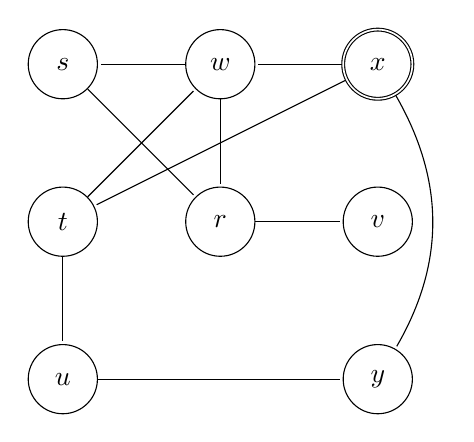
\begin{tikzpicture}[>=stealth',shorten >=1pt,auto,node distance=2cm]
  			\node[state, accepting]  (x) []           {$x$};
  			\node[state]             (w) [left of=x]  {$w$};
  			\node[state] 			 (s) [left of=w]  {$s$};
  			\node[state] 			 (r) [below of=w] {$r$};
  			\node[state]			 (v) [below of=x] {$v$};
  			\node[state]			 (t) [below of=s] {$t$};
  			\node[state]			 (u) [below of=t] {$u$};
  			\node[state]			 (y) [below of=v] {$y$};

  			\path[-] (x) edge (w)
             	         edge [bend left] (y)
             	         edge (t)
        	         (w) edge (r)
        	         	 edge (s)
        	         (s) edge (r)
        	         (t) edge (u)
        	         	 edge (w)
        	         (r) edge (v)
        	         (u) edge (y);
            	 		
		\end{tikzpicture}
	\end{center}
	
	To start running $BFS$ (Breadth First Search), all nodes that are adjacent to $x$ are inserted into $Q$. After inserting the nodes into $Q$, $G$ and $Q$ will look as follows:
	 
	
	\begin{center}
		$Q$ = [t,w,y]
		
		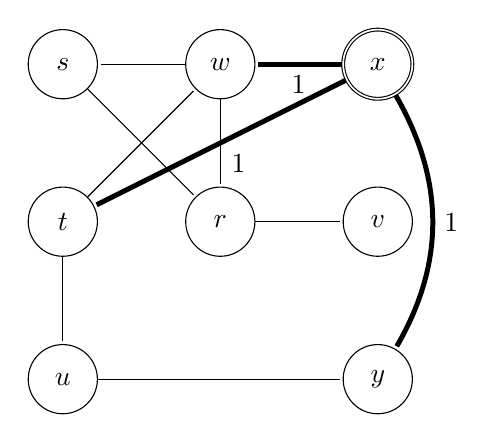
\begin{tikzpicture}[>=stealth',shorten >=1pt,auto,node distance=2cm]
  			\node[state, accepting]  (x) []           {$x$};
  			\node[state]             (w) [left of=x]  {$w$};
  			\node[state] 			 (s) [left of=w]  {$s$};
  			\node[state] 			 (r) [below of=w] {$r$};
  			\node[state]			 (v) [below of=x] {$v$};
  			\node[state]			 (t) [below of=s] {$t$};
  			\node[state]			 (u) [below of=t] {$u$};
  			\node[state]			 (y) [below of=v] {$y$};

  			\draw[-, line width=1.8pt] 
  					(x) edge node {1} (w)
             	        edge [bend left] node {1} (y)
             	        edge node {1} (t)
        	        (w) edge [thin] (r)
						edge [thin] (s)
					(s) edge [thin] (r)
					(t) edge [thin] (u)
						edge [thin] (w)
					(r) edge [thin] (v)
					(u) edge [thin] (y);
		\end{tikzpicture}		
	\end{center}

	Now that all the nodes that $x$ is adjacent too are added into $Q$, $t$ is dequeued from $Q$, $BFS$ branches out from the vertex $t$ to all adjacent nodes and adds them to $Q$.
	
	\begin{center}
		($Q$ \textbf{before} adding adjacent nodes of $t$) $Q$ = [w,y]
		
		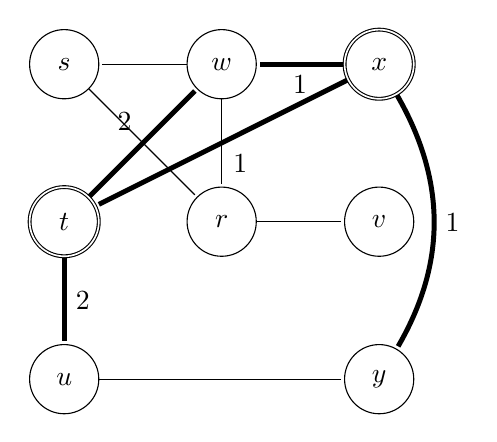
\begin{tikzpicture}[>=stealth',shorten >=1pt,auto,node distance=2cm]
  			\node[state, accepting]  (x) []           {$x$};
  			\node[state]             (w) [left of=x]  {$w$};
  			\node[state] 			 (s) [left of=w]  {$s$};
  			\node[state] 			 (r) [below of=w] {$r$};
  			\node[state]			 (v) [below of=x] {$v$};
  			\node[state, accepting]	 (t) [below of=s] {$t$};
  			\node[state]			 (u) [below of=t] {$u$};
  			\node[state]			 (y) [below of=v] {$y$};

  			\draw[-, line width=1.8pt] 
  					(x) edge node{1} (w)
             	        edge [bend left] node{1} (y)
             	        edge node{1} (t)
        	        (w) edge [thin] (r)
						edge [thin] (s)
					(s) edge [thin] (r)
					(t) edge node{2} (u)
						edge node{2} (w)
					(r) edge [thin] (v)
					(u) edge [thin] (y);
					
		\end{tikzpicture}	
		
		($Q$ \textbf{after} adding adjacent nodes of $t$) $Q$ = [w,y,u]	
	\end{center} 	
	
	We then repeat the same process that was performed with $t$ with the vertex $w$. 	
	
	\begin{center}
		($Q$ \textbf{before} adding adjacent nodes of $w$) $Q$ = [y,u]
		
		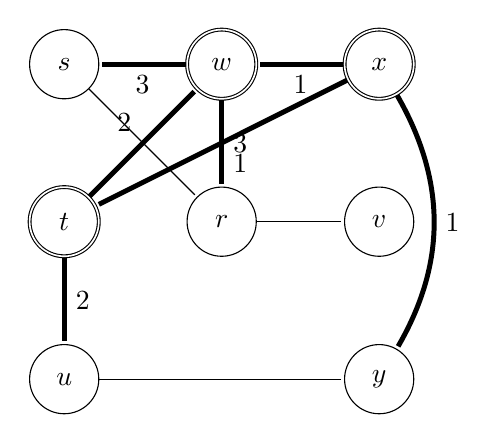
\begin{tikzpicture}[>=stealth',shorten >=1pt,auto,node distance=2cm]
  			\node[state, accepting]  (x) []           {$x$};
  			\node[state, accepting]  (w) [left of=x]  {$w$};
  			\node[state] 			 (s) [left of=w]  {$s$};
  			\node[state] 			 (r) [below of=w] {$r$};
  			\node[state]			 (v) [below of=x] {$v$};
  			\node[state, accepting]	 (t) [below of=s] {$t$};
  			\node[state]			 (u) [below of=t] {$u$};
  			\node[state]			 (y) [below of=v] {$y$};

  			\draw[-, line width=1.8pt] 
  					(x) edge node{1} (w)
             	        edge [bend left] node{1} (y)
             	        edge node{1} (t)
        	        (w) edge node{3} (r)
						edge node{3} (s)
					(s) edge [thin] (r)
					(t) edge node{2} (u)
						edge node{2} (w)
					(r) edge [thin] (v)
					(u) edge [thin] (y);
					
		\end{tikzpicture}	
		
		($Q$ \textbf{after} adding adjacent nodes of $w$) $Q$ = [y,u,r,s]	
	\end{center} 
 	
 	For the next iteration, we go $y$, and repeat the previous process.
 	
 	\begin{center}
		($Q$ \textbf{before} adding adjacent nodes of $y$) $Q$ = [u,r,s]
		
		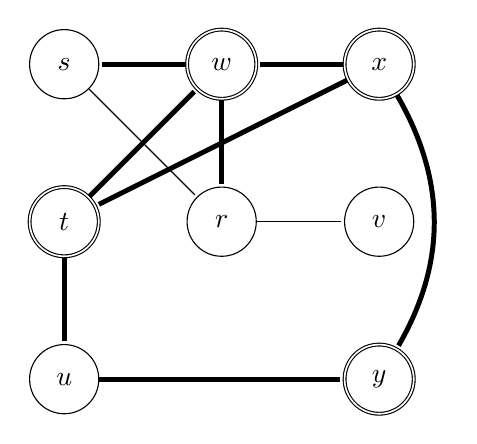
\begin{tikzpicture}[>=stealth',shorten >=1pt,auto,node distance=2cm]
  			\node[state, accepting]  (x) []           {$x$};
  			\node[state, accepting]  (w) [left of=x]  {$w$};
  			\node[state] 			 (s) [left of=w]  {$s$};
  			\node[state] 			 (r) [below of=w] {$r$};
  			\node[state]			 (v) [below of=x] {$v$};
  			\node[state, accepting]	 (t) [below of=s] {$t$};
  			\node[state]			 (u) [below of=t] {$u$};
  			\node[state, accepting]	 (y) [below of=v] {$y$};

  			\draw[-, line width=1.8pt] 
  					(x) edge (w)
             	        edge [bend left] (y)
             	        edge (t)
        	        (w) edge (r)
						edge (s)
					(s) edge [thin] (r)
					(t) edge (u)
						edge (w)
					(r) edge [thin] (v)
					(u) edge (y);
					
		\end{tikzpicture}	
		
		($Q$ \textbf{after} adding adjacent nodes of $y$) $Q$ = [u,r,s]	
	\end{center}  	
	
	Again, the process is repeated on the vertex $u$.
	
	\begin{center}
		($Q$ \textbf{before} adding adjacent nodes of $u$) $Q$ = [r,s]
		
		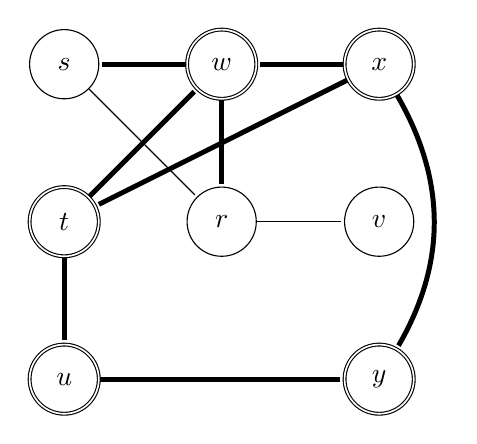
\begin{tikzpicture}[>=stealth',shorten >=1pt,auto,node distance=2cm]
  			\node[state, accepting]  (x) []           {$x$};
  			\node[state, accepting]  (w) [left of=x]  {$w$};
  			\node[state] 			 (s) [left of=w]  {$s$};
  			\node[state] 			 (r) [below of=w] {$r$};
  			\node[state]			 (v) [below of=x] {$v$};
  			\node[state, accepting]	 (t) [below of=s] {$t$};
  			\node[state, accepting]	 (u) [below of=t] {$u$};
  			\node[state, accepting]	 (y) [below of=v] {$y$};

  			\draw[-, line width=1.8pt] 
  					(x) edge (w)
             	        edge [bend left] (y)
             	        edge (t)
        	        (w) edge (r)
						edge (s)
					(s) edge [thin] (r)
					(t) edge (u)
						edge (w)
					(r) edge [thin] (v)
					(u) edge (y);
					
		\end{tikzpicture}	
		
		($Q$ \textbf{after} adding adjacent nodes of $u$) $Q$ = [r,s]. (\textbf{*NOTE} In this case, all adjacent nodes of $u$ were viewed, therefore no nodes were added to $Q$.	
	\end{center} 
	
	Moving forward from the previous iteration, the previous process is repeated on the vertex $r$.
	
	\begin{center}
		($Q$ \textbf{before} adding adjacent nodes of $r$) $Q$ = [s]
		
		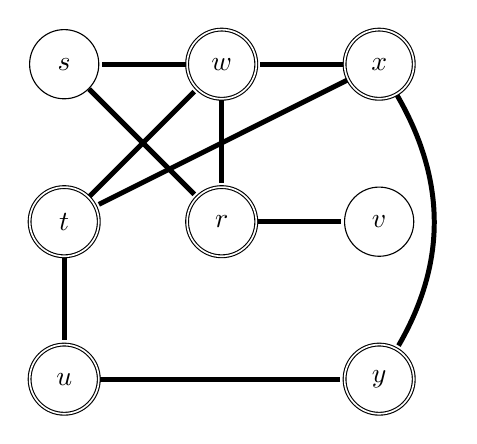
\begin{tikzpicture}[>=stealth',shorten >=1pt,auto,node distance=2cm]
  			\node[state, accepting]  (x) []           {$x$};
  			\node[state, accepting]  (w) [left of=x]  {$w$};
  			\node[state] 			 (s) [left of=w]  {$s$};
  			\node[state, accepting]  (r) [below of=w] {$r$};
  			\node[state]			 (v) [below of=x] {$v$};
  			\node[state, accepting]	 (t) [below of=s] {$t$};
  			\node[state, accepting]	 (u) [below of=t] {$u$};
  			\node[state, accepting]	 (y) [below of=v] {$y$};

  			\draw[-, line width=1.8pt] 
  					(x) edge (w)
             	        edge [bend left] (y)
             	        edge (t)
        	        (w) edge (r)
						edge (s)
					(s) edge (r)
					(t) edge (u)
						edge (w)
					(r) edge (v)
					(u) edge (y);
					
		\end{tikzpicture}	
		
		($Q$ \textbf{after} adding adjacent nodes of $r$) $Q$ = [s,v]. 
	\end{center} 
	
	Now, all edges have been seen by $BFS$, but all nodes have yet been visited, therefore, must continue running $BFS$ until $Q$ is empty. 	
	
	\begin{center}
		($Q$ \textbf{before} adding adjacent nodes of $s$) $Q$ = [v]
		
		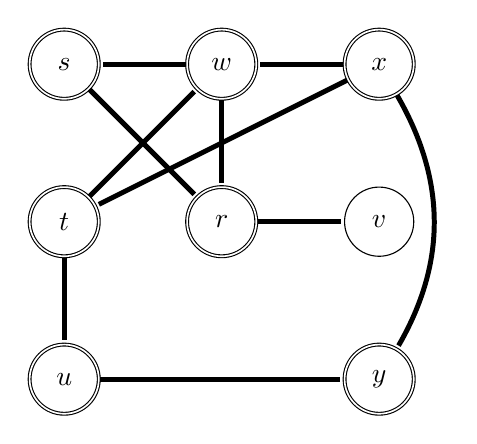
\begin{tikzpicture}[>=stealth',shorten >=1pt,auto,node distance=2cm]
  			\node[state, accepting]  (x) []           {$x$};
  			\node[state, accepting]  (w) [left of=x]  {$w$};
  			\node[state, accepting]  (s) [left of=w]  {$s$};
  			\node[state, accepting]  (r) [below of=w] {$r$};
  			\node[state]			 (v) [below of=x] {$v$};
  			\node[state, accepting]	 (t) [below of=s] {$t$};
  			\node[state, accepting]	 (u) [below of=t] {$u$};
  			\node[state, accepting]	 (y) [below of=v] {$y$};

  			\draw[-, line width=1.8pt] 
  					(x) edge (w)
             	        edge [bend left] (y)
             	        edge (t)
        	        (w) edge (r)
						edge (s)
					(s) edge (r)
					(t) edge (u)
						edge (w)
					(r) edge (v)
					(u) edge (y);
					
		\end{tikzpicture}	
		
		($Q$ \textbf{after} adding adjacent nodes of $s$) $Q$ = [v]. 
	\end{center} 
	
	\begin{center}
		($Q$ \textbf{before} adding adjacent nodes of $v$) $Q$ = [ ]
		
		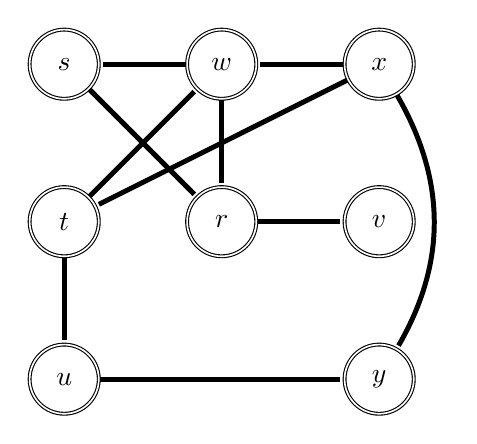
\begin{tikzpicture}[>=stealth',shorten >=1pt,auto,node distance=2cm]
  			\node[state, accepting]  (x) []           {$x$};
  			\node[state, accepting]  (w) [left of=x]  {$w$};
  			\node[state, accepting]  (s) [left of=w]  {$s$};
  			\node[state, accepting]  (r) [below of=w] {$r$};
  			\node[state, accepting]	 (v) [below of=x] {$v$};
  			\node[state, accepting]	 (t) [below of=s] {$t$};
  			\node[state, accepting]	 (u) [below of=t] {$u$};
  			\node[state, accepting]	 (y) [below of=v] {$y$};

  			\draw[-, line width=1.8pt] 
  					(x) edge (w)
             	        edge [bend left] (y)
             	        edge (t)
        	        (w) edge (r)
						edge (s)
					(s) edge (r)
					(t) edge (u)
						edge (w)
					(r) edge (v)
					(u) edge (y);
					
		\end{tikzpicture}	
		
		($Q$ \textbf{after} adding adjacent nodes of $v$) $Q$ = [ ]. 
	\end{center} 
	
	$Q$ is now empty and all nodes were visited. This concludes the process of $BFS$.

	\newpage	
	
	\textbf{Question 3: }Given a tree T=(V,E) compute its diameter, i.e. the longest path between two vertices. Do $BFS$ at a node $s$, find the farthest from $s$ to get a vertex, say $t$. Then do BFS to from $t$ to find the farthest from $t$. Prove this gives diameter of tree. Diameter of a tree is the longest path in the tree.
	
	\textbf{Answer 3: }
	
	\newpage		
	
	\textbf{Question 4: }Give an efficient algorithm that takes as input a directed graph G =(V,E) and and determines if there is a vertex s in V from which all other vertices can be reached.
	
	\textbf{Answer 4: }
	
	\newpage	
	
	\textbf{Question 5: }Show that in an undirected graph, the sum of the degrees of the vertices is twice the number of edges.
	
	\textbf{Answer 5: }

\end{document}